\documentclass[hyperref={pdfpagelabels=false}]{beamer}
\setbeamercolor{background canvas}{bg=white}
\usepackage{graphicx,lmodern,subfigure,ulem,color,graphicx,tikz,booktabs,natbib}
\usepackage{mathrsfs}
\usetheme{Warsaw}
%\definecolor{beamer@blendedblue}{rgb}{0.1,0.5,0.1}
%\definecolor{ForestGreen}{RGB}{60, 140, 60}
%\setbeamercolor{structure}{fg=beamer@blendedblue}
\setbeamertemplate{navigation symbols}{}
\setbeamertemplate{footline}[frame number]
\bibliographystyle{chicago}
\newcommand{\spitem}{\vspace{.3cm}\item}
\newcommand{\elas}{$E_{labor}$}
%\def \FigPath {Users\th3\Documents\Job_Market_Paper\Code\Figures} 
\DeclareMathOperator{\E}{\mathbb{E}}
\usepackage{makecell}




\title{Financial and Uncertainty Shocks}
\author{Marco Brianti}
\institute{Boston College}
\date{October 2018}

\usetheme[
outer/progressbar=foot,
outer/numbering=none
]{metropolis}


\begin{document}
	
	\frame{\titlepage \begin{center} Dissertation Project \end{center} }
	

	
	
		\frame{\frametitle{Alternative Drivers of Economic Fluctuations}
			
			\	
			
			\textit{The shocks that produced the recession were primarily associated with \textbf{financial disruptions} and \textbf{heightened uncertainty}}
			
			\hfill  Stock and Watson (2012) 
			%Stock and Watson (2012) comprehensive empirical anatomy of the Great recession
			%The shocks that produced the recession were primarily associated with financial disruptions and heightened uncertainty		
			
			
			\
			

			
Depth and duration of \textbf{financial crisis} 
\begin{itemize}
	\item[$\Rightarrow$] several challenges for standard business cycle models
\end{itemize}  
% who used traditional sources of BC fluctuations such as productivity shocks. In particular, those models together with those shocks were unable to explain important features specifically related to the financial crisis.

\

%In response to this limitation,		
New strands of literature arose proposing alternative shocks
\begin{enumerate}
	\item \textbf{Financial shocks} - Khan and Thomas (2013) JPE %among others Jerman and Quadrini (2012) AER, Christiano, Motto e Rostagno (2010) Working paper
	\item \textbf{Uncertainty shocks} - Bloom (2009) ECMA %was the first to estimate the dynamic effect of uncertainty in a both an empirical and theoretical context 
	\end{enumerate}

\




	}

	\frame{\frametitle{Theoretical Definitions}	
		
%Important to define because both shocks are residuals from endogenouse proxy variables that depends on other structural shocks	
\textbf{Financial Shocks.} Unanticipated innovations to financial conditions orthogonal to other economic disturbances.
$$
F_t = g(s_t^Y,s_t^U) + s_t^F
$$
\textit{E.g. new banking regulation, banks' balance sheet deterioration, changes in lenders' risk management, \dots}
%A financial shock is an unexpected deterioration of the credit conditions - in general proxied by the credit spread - which cannot be explained by other economic forces as productivity or policies. How can we think about s^F? Following Gilchrist (2012) AER, as a change in the risk-bearing capacity of the lending sector which is not trigger by other shocks. So s^F is a measure of our ignorance of the capital market, but it is an imortant one because it represents independent changes in the credit conditions. 

\

\



\textbf{Uncertainty Shocks.} Innovations to the forecast error variance of aggregate variables orthogonal to other economic disturbances.
$$
U_t = h(s_t^Y,s_t^F) + s_t^U
$$
\textit{E.g. political tension, terrorist attack, sectoral growth opportunities, \dots}
%when agents observe large 1st-order shocks they may also use this information to update the distribution of future shocks implying a jump in uncertainty. However, this jump is endogenous to a large realized shock. How can we think about s^U? According to Nimark (2014) - AER and Forni, Gambetti, and Sala (2017) - WP, I interpret s^U as a signal regarding future states of the economy which implies changes in the variance of the distribution of future shocks.

	
}
	
	
	\frame{\frametitle{Empirical Proxies for Financial Conditions and Uncertainty}	
		
		\
		
		\
		
			\begin{figure}
			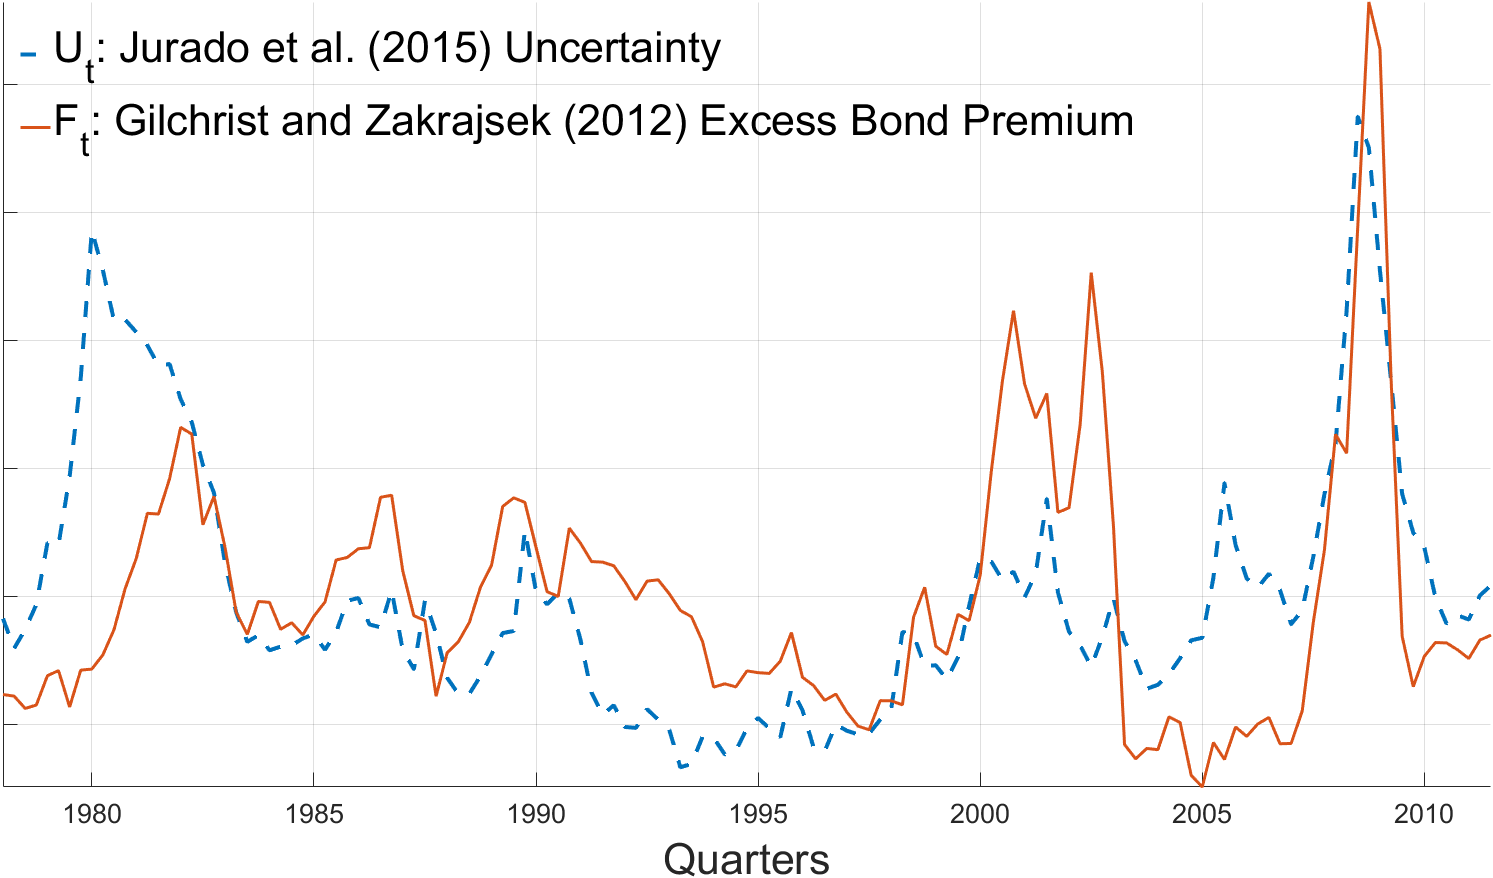
\includegraphics[scale=0.25]{Financial_Uncertainty}
			\label{fig:raw_data}
		\end{figure}
		
	}

	\frame{\frametitle{Motivation: Empirical Challenge in Structural VAR}	
	
	Empirically distinguishing between financial and uncertainty shocks is difficult
	\begin{itemize}
		\item[$\Rightarrow$] financial distress is empirically associated with larger volatility 
	\end{itemize}

\


Within a SVAR framework, this correlation significantly complicates identification of both shocks
\begin{enumerate}
	\item Implausible \textbf{zero-contemporaneous restrictions}
	\begin{itemize}
		\item[$\Rightarrow$] Both $F_t$ and $U_t$ are fast moving
	\end{itemize}	
	\item Unavailable instruments for \textbf{sign restrictions}	
	\begin{itemize}
		\item[$\Rightarrow$] Current theoretical models predict same qualitative effects on both prices and quantities
	\end{itemize}
\end{enumerate}
	
	
}





\frame{\frametitle{My contribution}
	
	I want to take a step back and show evidence and theory that financial and uncertainty shocks are \textbf{qualitative different}.
	
	
	\
		
	
	
	
	In particular, 
	
	
	\begin{enumerate}
		\item \textbf{Corporate cash holdings} respond differently to financial and uncertainty shocks. 
		\begin{itemize}
			\item[$\Rightarrow$] Identification assumption
			\end{itemize}
		
		\	
		
		\item I provide a \textbf{new econometric tool} to simultaneously identify two structural shocks when an internal instrument is available.\begin{itemize}
			\item[$\Rightarrow$] Generalized Penalty Function Approach  
		\end{itemize}
		
	\end{enumerate}
}

\frame{\frametitle{Roadmap}
	\Large{
		$ \ \ \ \ \ $ 1. \textbf{Cash Holdings}
		
		$ \ \ \ \ \ $ 2. Model
		
		$ \ \ \ \ \ $ 3. Empirical Strategy
		
		$ \ \ \ \ \ $ 4. Results
		
		$ \ \ \ \ \ $ 5. Conclusions
	}
}
	

\frame{\frametitle{Corporate Cash Holdings}
	
	\
	
\textbf{Cash and Cash Equivalents} refer to assets a business holds as ready cash
\begin{itemize}
	\item Coffer as petty cash
	\item Bank account
	\item Bank certificates of deposits
\end{itemize}

\

U.S. large firms have cash equal to about 15\% of total assets.

\

It is a \textbf{stock variable}, 
$$
Cash_t = Cash_{t-1} + NY_t + \delta K_t - I_t + B_t - D_t.
$$




}


\frame{\frametitle{Cash is a Substitute for External Finance}
	
	

	\begin{itemize}
	\item[1.] Financially constrained firms use cash as an \textbf{internal source of investment funding}.
	
	\hfill Kaplan and Zingales, 1997 QJE
\end{itemize}


		

	\begin{itemize}
	\item[2.] Financially constrained firms \textbf{store cash in good times} and \textbf{use it in bad ones}.
	
	\hfill Almeida, Campello, Weisbach, 2004 JF 	
\end{itemize}
	
		

	\begin{itemize}
	\item[3.] After a negative credit supply shock firms \textbf{burn cash} to \textbf{avoid investment cuts} and \textbf{reduce financial costs}.
	
	\hfill Campello, Graham, Harvey, 2010 JFE
\end{itemize}

	

	\begin{itemize}
	\item[4.] At a country level, \textbf{cash-to-assets is positively correlated to credit-to-GDP}.
	
	\hfill Lins, Servaes, Tufano (2010) JFE
\end{itemize}

	

		
	
}

		\frame{\frametitle{Cash is Positively Correlated with Uncertainty}
				\begin{itemize}
				\item[1.] Financially constrained firm \textbf{holds more cash if cash flow is more volatile}.

\hfill Han and Qiu (2007) JCF
\end{itemize}

					\begin{itemize}
		\item[2.] Firms \textbf{increase their liquidity ratios when macroeconomic uncertainty increases}.
		
		\hfill Baum, Coglayan, Stephan, Talavera (2008) EM	
	\end{itemize}		

					\begin{itemize}
	\item[3.] Using UK data, they show that \textbf{cash is positively associated to higher uncertainty}.
	
	\hfill Bloom, Mizen, Smietanka (2018) WP	
\end{itemize}			
	


					\begin{itemize}
	\item[4.] In response to an \textbf{uncertainty shock}, firms \textbf{increase cash reserves}.
	
	\hfill Alfaro, Bloom, Lin (2018) NBER WP	
\end{itemize}	
	
}

\frame{\frametitle{Roadmap}
	\Large{
		$ \ \ \ \ \ $ 1. Cash Holdings
		
		$ \ \ \ \ \ $ 2. \textbf{Model}
		
		$ \ \ \ \ \ $ 3. Empirical Strategy
		
		$ \ \ \ \ \ $ 4. Results
		
		$ \ \ \ \ \ $ 5. Conclusions
	}
}
	
	
%\frame{\frametitle{Economic Intuition I}	
		
%To provide an economic intuition of the differential response of \textbf{cash holdings} to uncertainty and financial shocks, I present a properly augmented model in the spirit of 
%\begin{itemize}
	%\item Almeida, Campello, and Weisbach (2004)
	%\item Han and Qiu (2007)
%\end{itemize}

%\

%It is a simple representation of a dynamic setting where a credit-constrained profit-maximizing firm has a trade-off between present and future investment opportunities
		
%}

\frame{\frametitle{Three-Period Partial Equilibrium Model}
	
	

\begin{itemize}
	\item[]
\begin{itemize}
     \item[Period 0] $ \ \ \ d_0 = y_0 + b_0 - i_0 - c$
	
	\
	
	
	\item[Period 1] $ \ \ \ d_1 = y_1 + b_1 - i_1 + c, \ \ \ $ where $ \ y_1 \sim F(y_0,\sigma^2)$
	
	\
	
	
	\item[Period 2] $ \ \ \ d_2 = g(i_0) - b_0(1 + r_0) + g(i_1) - b_1(1 + r_1)$
\end{itemize}
\end{itemize}

\begin{eqnarray*}
	\begin{aligned}
\max_{\{ b_t,i_t,c \}_{t=0,1}} \ \ &\E \Big[  d_0 + d_1 + d_2     \Big| F  \Big] \\
\text{subject to} \ \ &r_0 = \frac{1}{2}\alpha_0 b_0 \ \ \text{and} \ \ r_1 = \frac{1}{2}\alpha_1 b_1 \\
&d_t \geq 0, \ \ \ t = 0,1,2
\end{aligned}
\end{eqnarray*}

\

\begin{center}
Financial shock: $\uparrow \alpha_0$ $ \ \ \ \ $ vs $ \ \ \ \ $ Uncertainty shock: $\uparrow \sigma^2$
\end{center}
	
}


\frame{\frametitle{Solution}
	
	Firm needs external finance: $\E_0 \Big[ g(y_t) \Big] > 1$ for $t=0,1$
\begin{itemize}
	\item[$\Rightarrow$] $d_t = 0 \ \ $ for $ \ t=0,1$
\end{itemize}
which implies $i_0 = y_0 + b_0 - c$ and $i_1 = y_1 + b_1 + c$. Objective function is,
\begin{eqnarray*}
	\begin{aligned}
	\max_{b_0,b_1,c} \ \ &g \big( i_0 \big) - b_0 - \frac{1}{2} \alpha_0 b_0^2 - y_0 + \E \bigg[  g \big( i_1 \big) - b_1 - \frac{1}{2} \alpha_1 b_1^2 - y_1   \bigg| F     \bigg]
	 \end{aligned}
	\end{eqnarray*}
First Order Conditions
\begin{itemize}
	\item[$b_0:$] $g'(y_0 + b_0^* - c^*) = 1 + \alpha_0 b_0^*$
	
	
	\item[$b_1:$] $\E \Big[ g'(y_1 + b_1^* + c^*) \Big] = 1 + \alpha_1 b_1^*$
	
	
	
	\item[$c:$] $\E \Big[ g'(y_1 + b_1^* + c^*) \Big] = g'(y_0 + b_0^* - c^*)$
\end{itemize}

}

\frame{\frametitle{Comparative Statics}
	
	Given the first order conditions,
\begin{itemize}
	\item[$b_0:$] $g'(y_0 + b_0^* - c^*) = 1 + \alpha_0 b_0^*$
	
	
	\item[$b_1:$] $\E \Big[ g'(y_1 + b_1^* + c^*) \Big] = 1 + \alpha_1 b_1^*$
	
	
	
	\item[$c:$] $\E \Big[ g'(y_1 + b_1^* + c^*) \Big] = g'(y_0 + b_0^* - c^*)$
\end{itemize}

\
	
\textbf{Uncertainty shock}: $y_1 \sim Q$ which is mean-preserving spread in $F$
	\begin{enumerate}
	\item[$\Rightarrow$] $c^*(\alpha_0,Q) > c^*(\alpha_0,F)$ as long as $g'''(\cdot) > 0$
\end{enumerate}

\

\textbf{Financial shock}: $\alpha_0^f > \alpha_0$ which is an exogenous increase in $r_0$
	\begin{enumerate}
	\item[$\Rightarrow$] $c^*(\alpha_0^f,F) < c^*(\alpha_0,F)$ 
\end{enumerate}



}



\frame{\frametitle{Roadmap}
	\Large{
		$ \ \ \ \ \ $ 1. Cash Reserves
		
		$ \ \ \ \ \ $ 2. Model
		
		$ \ \ \ \ \ $ 3. \textbf{Empirical Strategy}
		
		$ \ \ \ \ \ $ 4. Results
		
		$ \ \ \ \ \ $ 5. Conclusions
	}
}












\frame{\frametitle{Empirical Analysis}
	
	\

Given the reduced-form system $X_t = B X_{t-1} + \iota_t$ where

$$
X_t = \begin{bmatrix}
U_t \\
F_t \\
GDP_t \\
C_t \\
I_t \\
H_t \\
C2A_t 
\end{bmatrix}
$$ 

\

\begin{itemize}
	\item where $\iota_t' \iota_t = \Sigma_{\iota}$
	\item dataset ranges from 1986q1 to 2015q4
\end{itemize}

	
}





\frame{\frametitle{Sequential Penalty Function Approach}
	
	\
	
	\textbf{Step 1 - Uncertainty Shock}
	\begin{eqnarray*}
		\begin{aligned}
		\max_{\gamma_{U}} \ \ \ \ \ &  \ \underbrace{e_U A_0 \gamma_U}_{\text{Impact on U}} \ \ \  + \ \ \ \textcolor{red}{\delta} \underbrace{e_{C} A_0 \gamma_U}_{\text{Impact on Cash}} \\
		\text{subject to} \ \ \ \ \  & \ \delta \geq 0 \ \ \ \ \ \ \text{and} \ \ \ \ \ \  \underbrace{\gamma_U \gamma_U' = 1}_{\text{Normalization}}
		\end{aligned}
	\end{eqnarray*}

\



	\textbf{Step 2 - Financial Shock}
	\begin{eqnarray*}
		\begin{aligned}
		\max_{\gamma_{F}} \ \ \ \ \ & \  \underbrace{e_F A_0 \gamma_F}_{\text{Impact on F}} \ \ \  - \ \ \  \textcolor{red}{\delta} \underbrace{e_{C} A_0 \gamma_F}_{\text{Impact on Cash}} \\
		\text{subject to} \ \ \ \ \ \ & \ \delta \geq 0, \ \ \ \ \ \ \ \underbrace{\gamma_F \gamma_F' = 1}_{\text{Normalization}}, \ \ \ \ \ \ \text{and} \underbrace{\textcolor{red}{\gamma_U \gamma_F' = 0}}_{\text{Orthogonality with U shock}}
		\end{aligned}
	\end{eqnarray*}
	
}

\frame{\frametitle{A Novel Approach}

I suggest a \textbf{general approach} where $\delta$ is treated as an endogenous parameter chosen by the data.
\begin{itemize}
\item[$\Rightarrow$] Given the problem above, set $\delta$ such that $\gamma_U \gamma'_F = 0$
\end{itemize}

\begin{center}
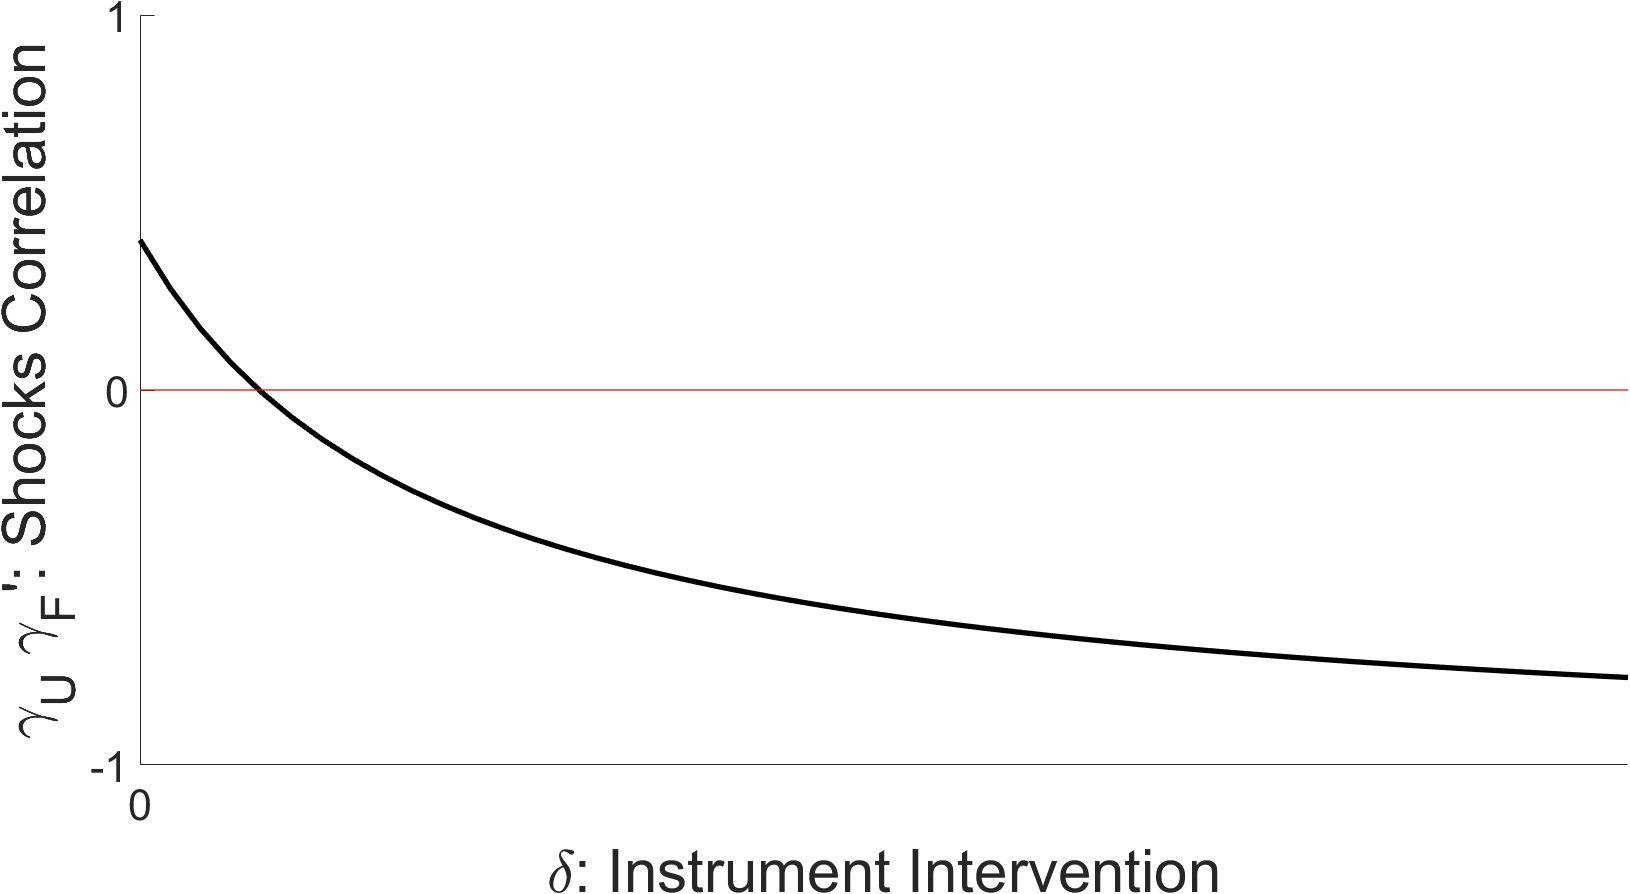
\includegraphics[scale=0.18]{fig_GPFA_intuition_figure_}
\end{center}

\textbf{Intuition.} Weight of the internal instrument should be large enough such that $\gamma_U \gamma_F' = 0$ endogenously holds.

}

\frame{\frametitle{Roadmap}
	\Large{
		$ \ \ \ \ \ $ 1. Cash Reserves
		
		$ \ \ \ \ \ $ 2. Model
		
		$ \ \ \ \ \ $ 3. Empirical Strategy
		
		$ \ \ \ \ \ $ 4. \textbf{Results}
		
		$ \ \ \ \ \ $ 5. Conclusions
	}
}

\frame{\frametitle{Uncertainty Shock}

\begin{center}
	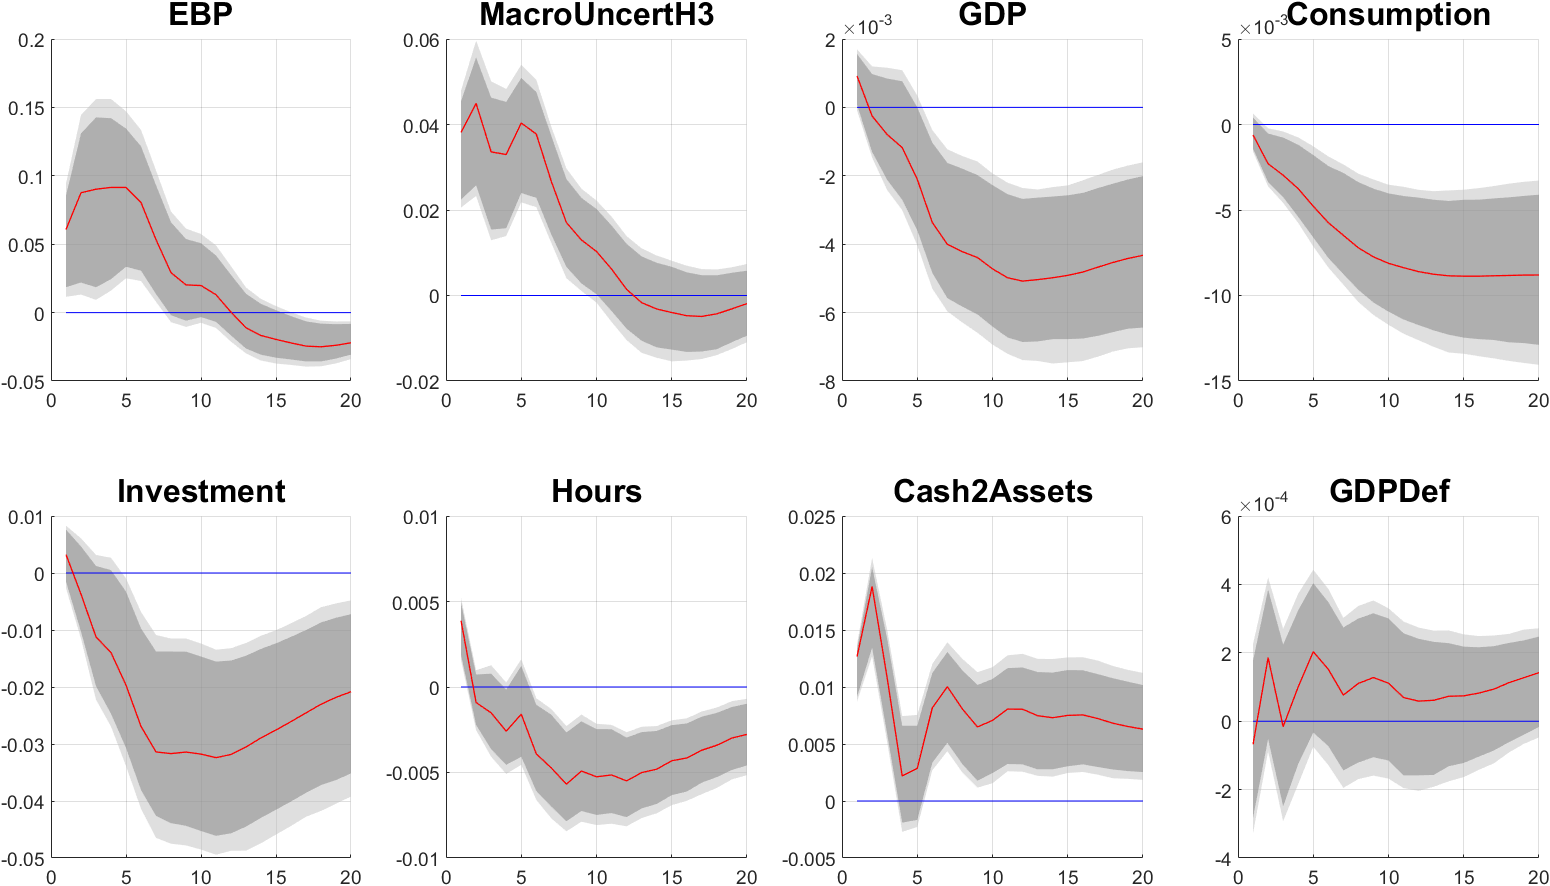
\includegraphics[scale=0.27]{fig_Uncertainty_Shock_GPFA_Compustat_3lags_gamgamZero}
\end{center}	

	
}

\frame{\frametitle{Financial Shock}
	
	\begin{center}
		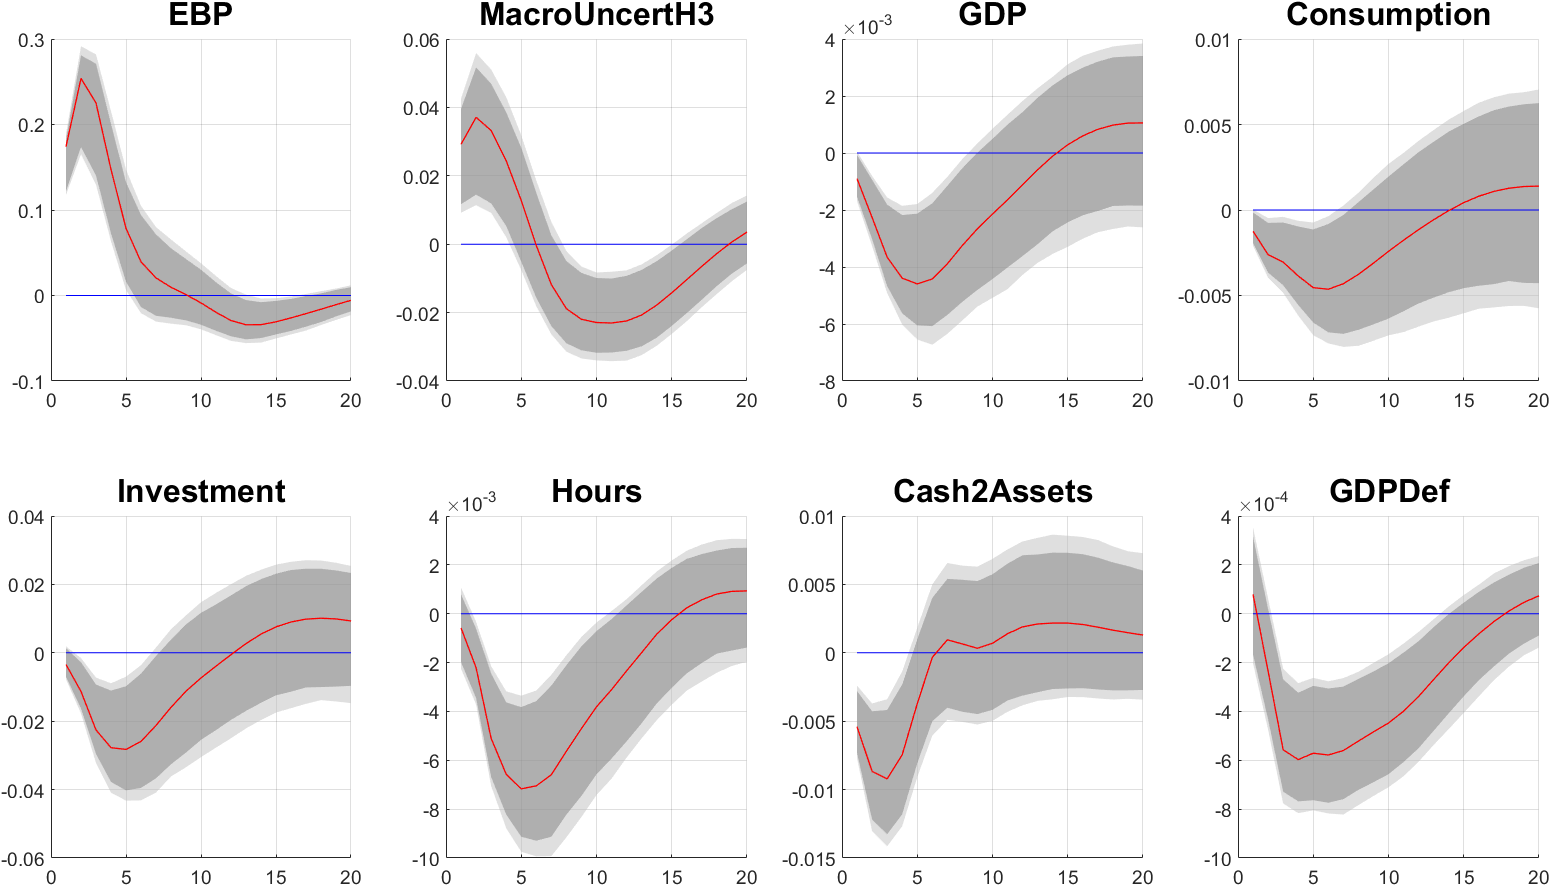
\includegraphics[scale=0.27]{fig_Financial_Shock_GPFA_Compustat_3lags_gamgamZero}
	\end{center}	
		
}



\frame{\frametitle{Variance Explained}
	
	\begin{center}
		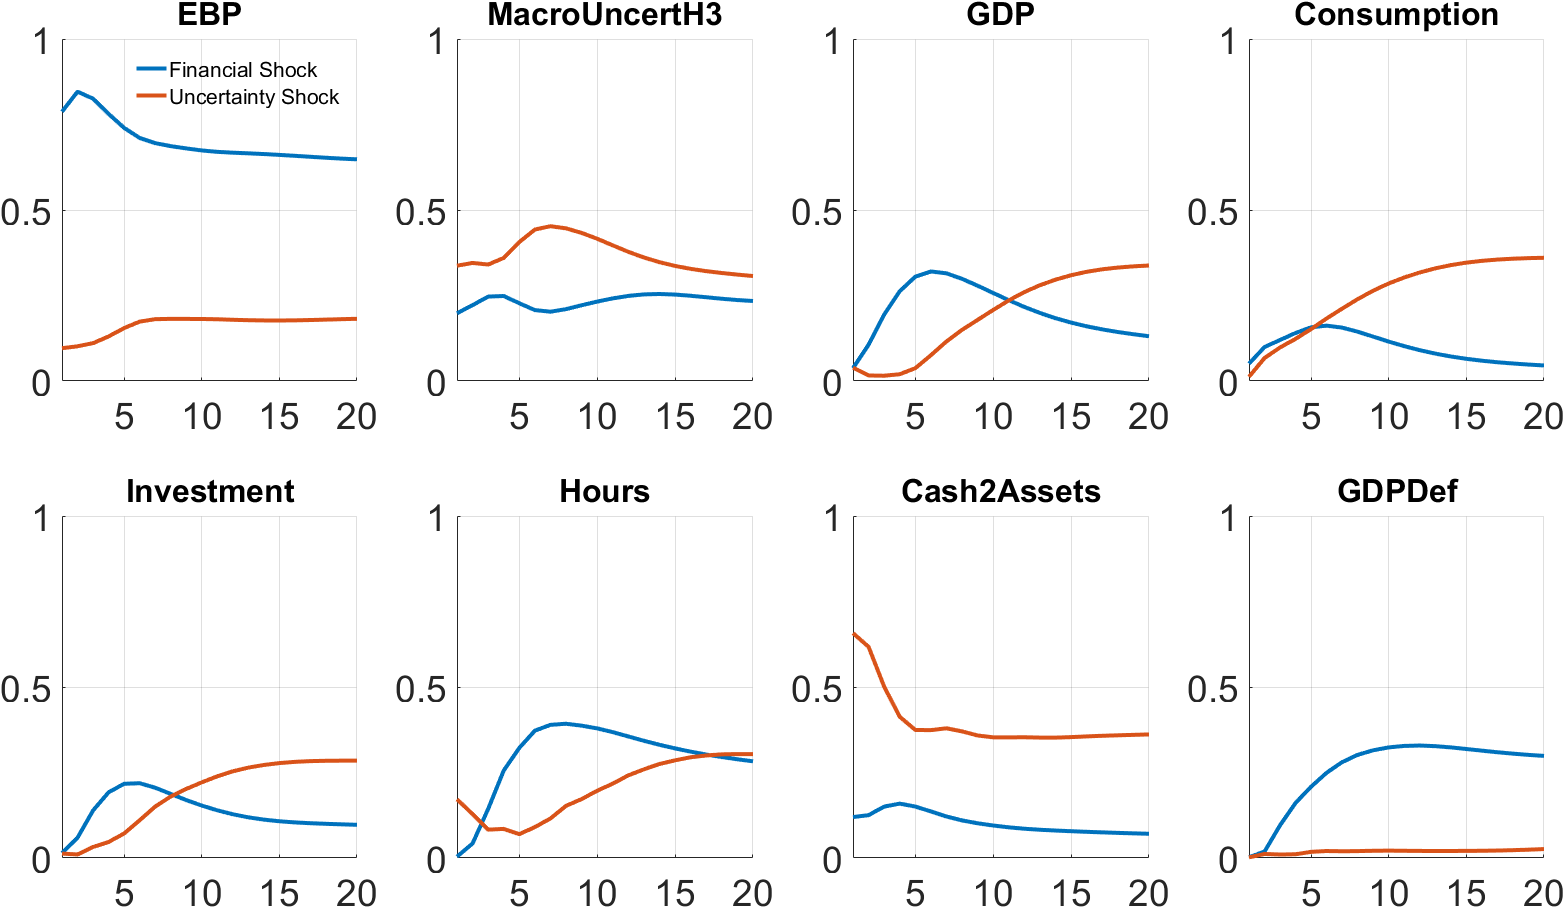
\includegraphics[scale=0.27]{fig_var_dec_vardec_GPFA_Compustat_3lags_gamgamZero}
	\end{center}	
	
}

\frame{\frametitle{Roadmap}
	\Large{
		$ \ \ \ \ \ $ 1. Cash Reserves
		
		$ \ \ \ \ \ $ 2. Model
		
		$ \ \ \ \ \ $ 3. Empirical Strategy
		
		$ \ \ \ \ \ $ 4. Results
		
		$ \ \ \ \ \ $ 5. \textbf{Conclusions}
	}
}

\frame{\frametitle{Conclusions}
	
So far,
	
\begin{itemize}
	
\item Cash as an internal instrument to simultaneously identify financial and uncertainty shocks


\item An econometric tool to overcome known SVAR shortcomings
\begin{itemize}
	\item[$\Rightarrow$] Simulated data confirm the reliability of the procedure 
\end{itemize}


\item Empirical results confirm the relevance of both shocks


\item Financial shocks have larger effects in the short run while uncertainty shocks in the medium run

\end{itemize}

	Nest Steps,
\begin{itemize}
	
	\item Firm-level evidence on the differential response of cash
	
	\item General equilibrium model
	
\end{itemize}

}

\frame{\frametitle{Appendix A - Simulated Data}
	
	Consider the following structural model,
	
	\begin{itemize}
		\item $U_t = B_{UU} U_{t-1} + B_{UF} F_{t-1}  + B_{UC} C_{t-1}  +  \underbrace{A_{UU}s_t^U  +  A_{UF}s_t^F}_{\text{$\iota_t^U$}}$
		\item $F_t = B_{FU} U_{t-1} + B_{FF} F_{t-1}  + B_{FC} C_{t-1}  +  \underbrace{A_{FU}s_t^U  +  A_{FF}s_t^F}_{\text{$\iota_t^F$}}$
		\item $C_t = B_{CU} U_{t-1} - B_{CF} F_{t-1}  + B_{CC} C_{t-1}  +  \underbrace{A_{CU}s_t^U  -  A_{CF}s_t^F}_{\text{$\iota_t^C$}}$
		\end{itemize}

	
	Objective is to estimate $s_t^U$ and $s_t^F$ under the assumption that we just know the sign of each element of $A$.
	
	\
	
	I apply the GPF approach - as shown previously - on simulated data.
	
}


\frame{\frametitle{Appendix A - Result for T = 100}
	
\begin{center}
	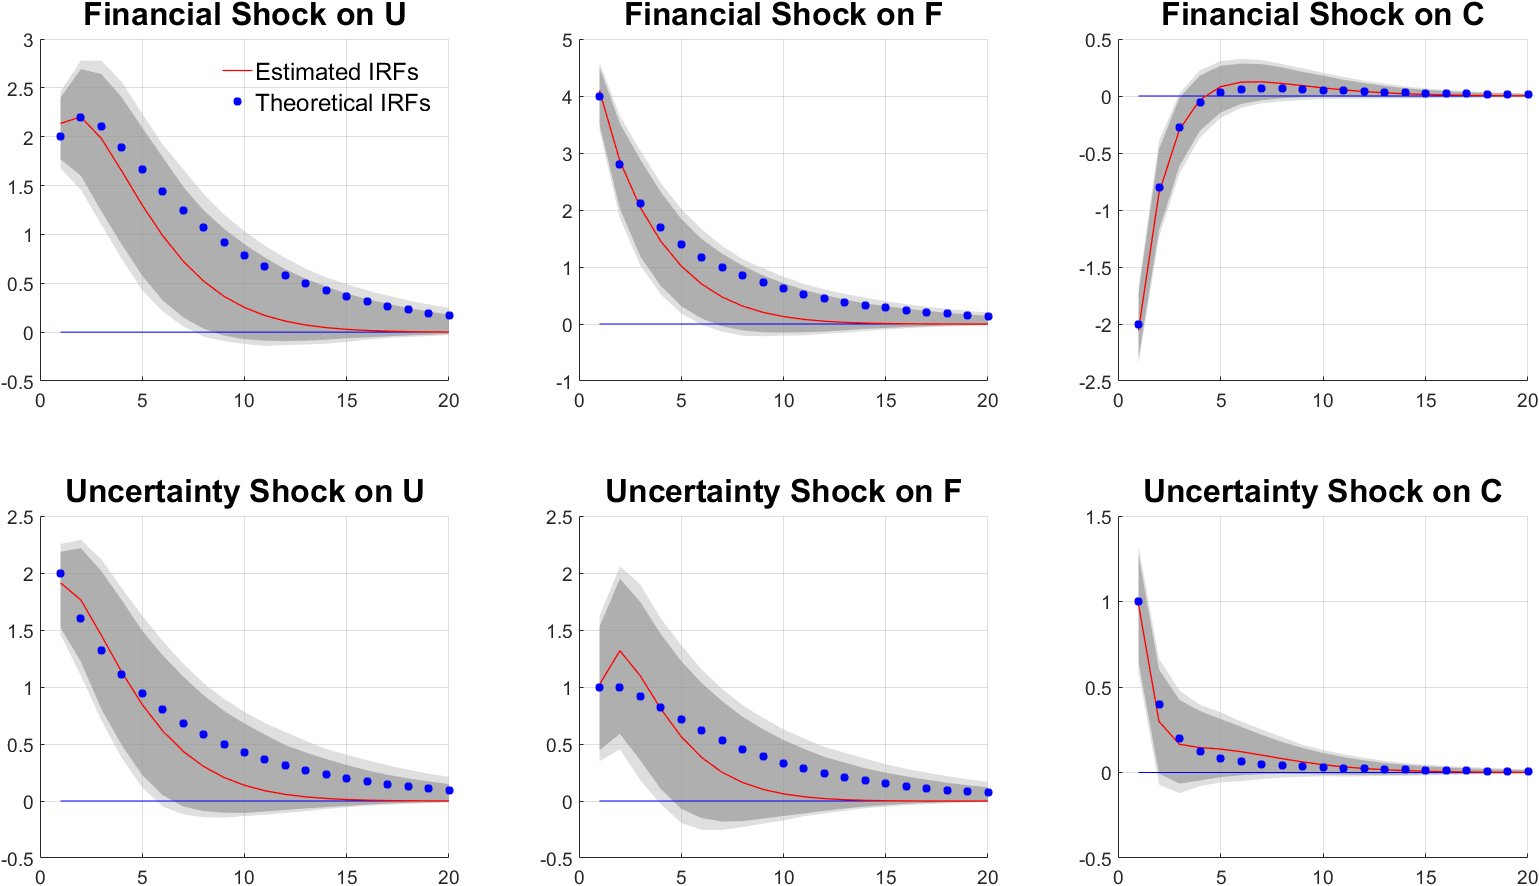
\includegraphics[scale=0.27]{test_small}
\end{center}	

	
}



\frame{\frametitle{Appendix A - Result for T = 100000}
	
\begin{center}
	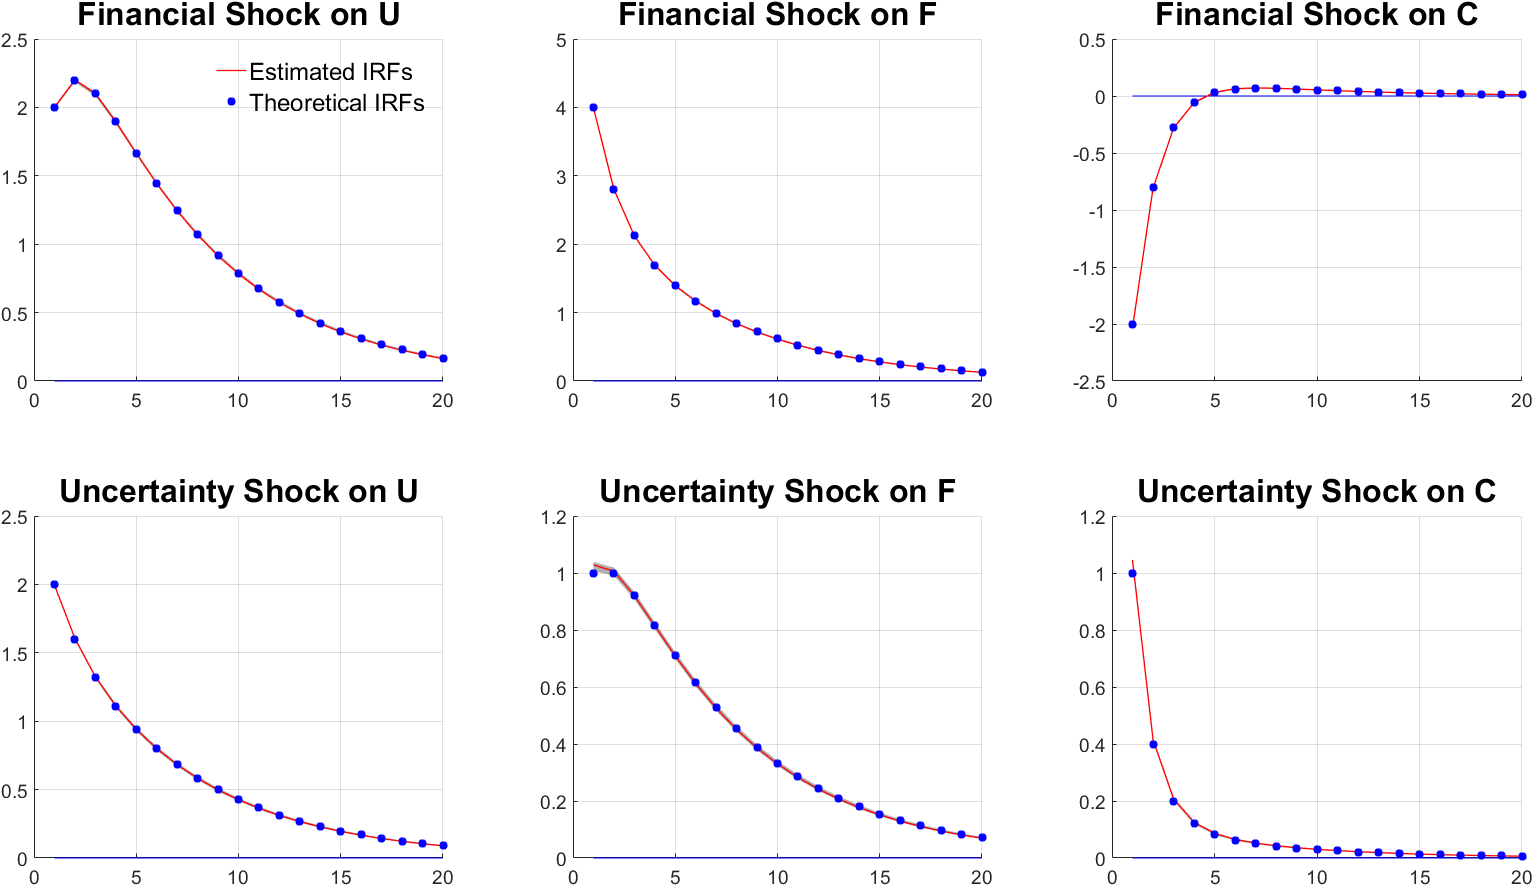
\includegraphics[scale=0.27]{test_large}
\end{center}		
	
}


\frame{\frametitle{Appendix B - Correlations with Other External Shocks}
	
	
	\begin{table}[h!]
		\centering
		\begin{tabular}{lrr} \hline \hline
			                & \textbf{Uncertainty Shocks} & \textbf{Financial Shocks} \\ 
			                \hline
			\textit{External Shocks} &                    &                      \\ 
			BZP Military News        & $-0.10$  $(0.24)$  &   $0.08$  $(0.31)$   \\ 
			Ramey Military news      &  $0.07$  $(0.44)$  &   $0.02$  $(0.82)$   \\ 
			LWY Exp. Tax             &  $0.03$  $(0.74)$  &   $0.15$  $(0.11)$   \\ 
			RRMR Unexp. Tax          & $-0.13$  $(0.16)$  &   $0.05$  $(0.59)$   \\ 
		    RRMR Exp. Tax            & $-0.08$  $(0.36)$  &   $0.03$  $(0.76)$   \\ 
		    AdjTFP AR(1)             &  $0.08$  $(0.31)$  &  $-0.14$  $(0.11)$   \\ 
		    RR Mon. Policy           & $-0.13$  $(0.18)$  &  $-0.04$  $(0.70)$   \\ 
		    \hline \hline
		\end{tabular}
	\end{table}
		
	
}













\end{document}